\section{Partiolaisuuden aakkoset}

\textit{Samoajavartio Vene listasi omat partiolaisuuden aakkosensa kevään 
2024 kokouksessaan. Kuinka hyvin nämä kuvaisivat juuri sinua?}

\begin{multicols}{3}
\setlength{\parindent}{0em}\setlength{\parskip}{.5em} {\large A}ina valmiina

{\large B}alansoitunut

{\large C}harmikas

{\large D}emokraattinen

{\large E}nerginen

{\large F}unktionaalinen

{\large G}uru

{\large H}ilpeä

{\large I}nnovatiivinen

{\large J}ohtaja

{\large K}ajahtanut

{\large L}uova

{\large M}onipuolinen

{\large N}ero

{\large O}ppivainen

{\large P}ystyvä

{\large Q}uadrifoglio

{\large R}eipas

{\large S}uvaitseva

{\large T}ietäväinen

{\large U}telias

{\large V}almis

{\large W}atti

{\large X}-treme leiriytyjä

{\large Y}ritteliäs

{\large Z}en

{\large Å}hå

{\large Ä}lykäs

{\large Ö}veri
\end{multicols}

\begin{figure}[!h]
\centering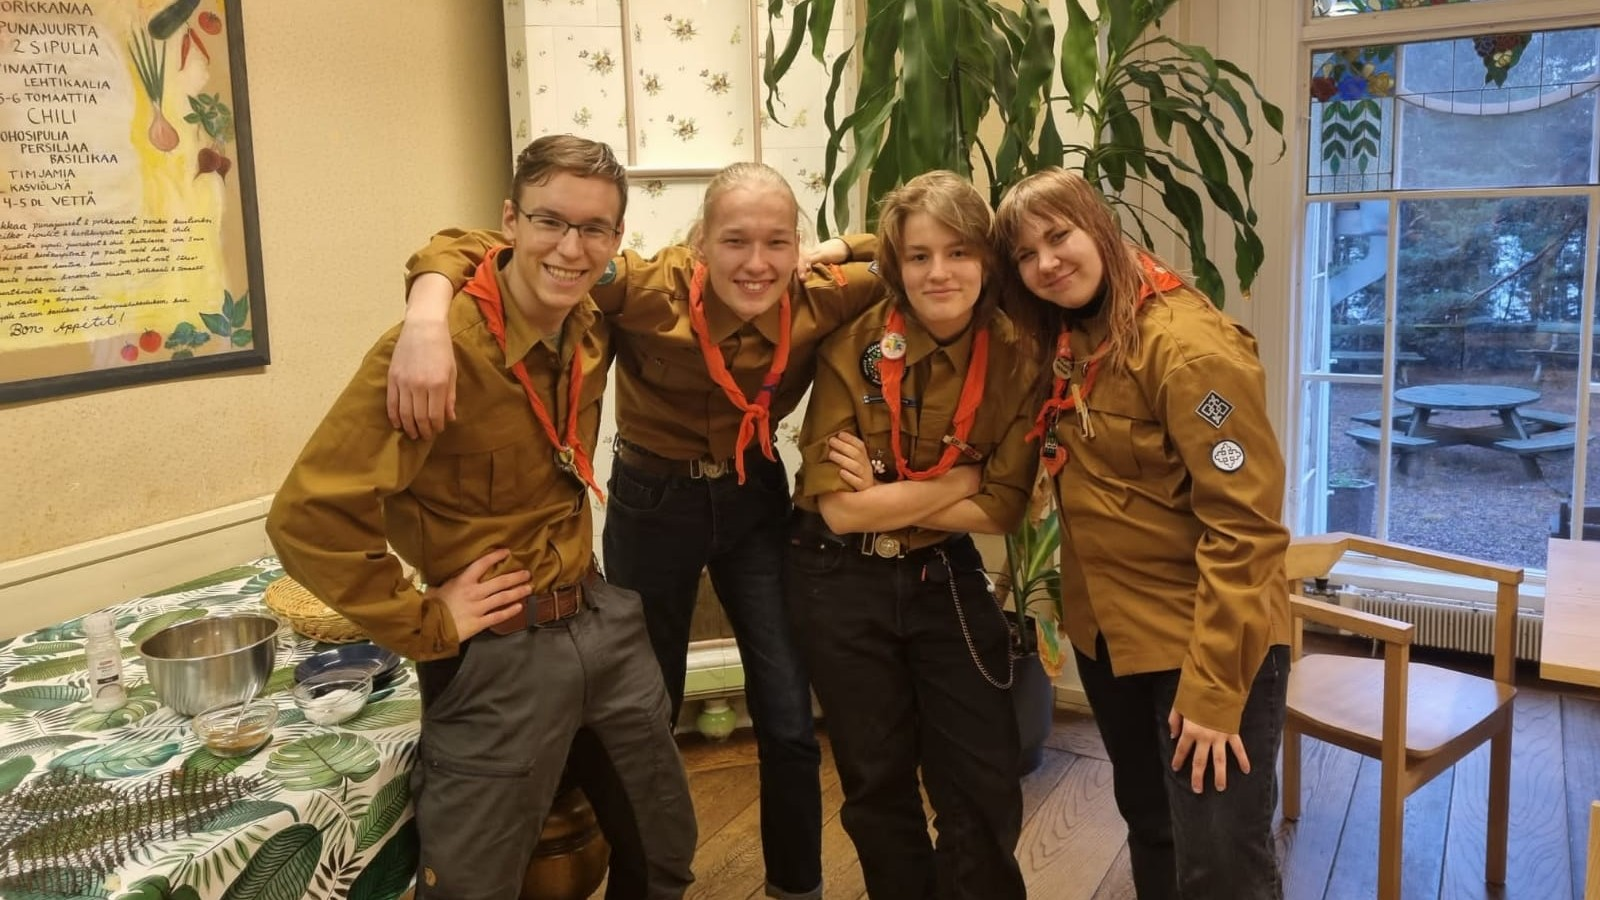
\includegraphics[width=\textwidth]{assets/vene}
\caption{\textit{Vene}-vartio.}
\end{figure}

\medskip

\noindent\null\hfill Kuva: Nonna
